\documentclass[a4paper,11pt]{article}
\usepackage{tikz}
\usepackage{times}
\usetikzlibrary{automata}
\usetikzlibrary{shapes}
\pagestyle{empty}
\usepackage{vmargin}
\tikzstyle{unobs}=[circle,draw=black,fill=white,thick,minimum width=1.4cm, minimum height=1.4cm]
\tikzstyle{obs}=[circle,draw=black,fill=lightgray,thick,minimum width=1.4cm, minimum height=1.4cm]

\setpapersize{custom}{11cm}{4cm}
\setmarginsrb{0cm}{0.0cm}{0cm}{0cm}{0cm}{0cm}{0cm}{0cm}

\begin{document}
\newcommand{\vbullets}[1]{% vertical bullets
\node[rectangle,anchor=center,at=(#1),text width=2ex]{%
$\bullet$\\[-1ex] $\bullet$\\[-1ex] $\bullet$}
}%

\begin{center}
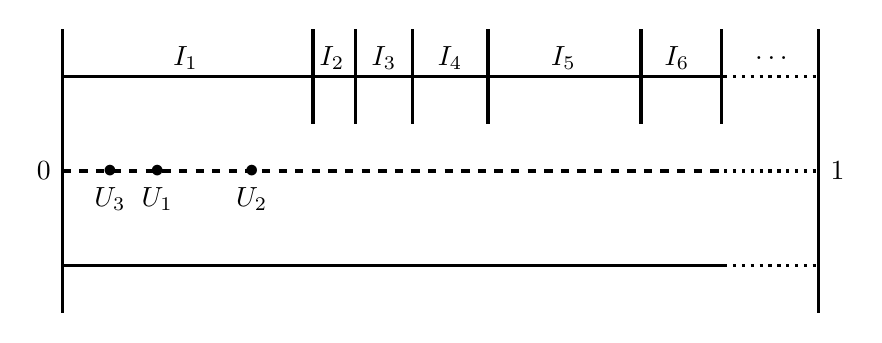
\begin{tikzpicture}[x=1.2cm,y=1.2cm,very thick,>=latex,baseline=(current bounding box.center)]
\tikzstyle{initial}=[ultra thick]
\draw (0,2.5) -- (0,5.5);
\draw (8,2.5) -- (8,5.5);
\draw (0,5) -- (7,5);
\draw[dotted] (7,5) -- (8,5);

\draw (0,4)[dashed] -- (7,4);
\draw[dotted] (7,4) -- (8,4);

\draw (0,3) -- (7,3);
\draw[dotted] (7,3) -- (8,3);
\node[rectangle] at (0.5,4) {$\bullet$};

\node at (0.5,3.7) {$U_3$};
\node[rectangle] at (1,4) {$\bullet$};
\node at (1,3.7) {$U_1$};
\node[rectangle] at (2,4) {$\bullet$};
\node at (2,3.7) {$U_2$};

\draw (6.97,4.5) -- (6.97,5.5);
\draw (6.12,4.5) -- (6.12,5.5);
\draw (4.5,4.5) -- (4.5,5.5);
\draw (3.7,4.5) -- (3.7,5.5);
\draw (3.1,4.5) -- (3.1,5.5);
\draw (2.65,4.5) -- (2.65,5.5);

\node (t1) at (-0.2,4) {0};
\node (t1) at (8.2,4) {1};
\node (t1) at (7.5,5.2) {$\ldots$};
\node (t1) at (6.5,5.2) {$I_6$};
\node (t1) at (5.3,5.2) {$I_5$};
\node (t1) at (4.1,5.2) {$I_4$};
\node (t1) at (3.4,5.2) {$I_3$};
\node (t1) at (2.85,5.2) {$I_2$};
\node (t1) at (1.3,5.2) {$I_1$};




\end{tikzpicture}
\end{center}
\end{document}
